%!TeX root=../main.tex
\فصل{پروتکل‌های ارتباطی}
\قسمت{مقدمه}
قطعات الکترونیک نیز همانند انسان‌ها برای ارتباط با یکدیگر باید از یک زبان واحد قابل‌فهم برای هر دو طرف استفاده کنند که به این زبان‌ها پروتکل‌های ارتباطی گفته می‌شود. در این پروژه نیز همانند اکثر پروژه‌های الکترونیکی از تعدادی از این پروتکل‌ها برای برقراری ارتباط بین قطعات الکترونیکی مختلف (سنسورها، فرستنده-گیرنده‌های رادیویی و میکروکنترلر) استفاده شده است. در زیر اطلاعات کلی هر یک از پروتکل‌های ارتباطی استفاده‌شده در این پروژه آمده است.

\قسمت{پروتکل \متن‌لاتین{SPI}}

این پروتکل یک رابط ارتباط سریالی سنکرون\پانویس{synchronous} (همزمان) چهار سیم است که برای ارتباط بین تنها یک \متن‌لاتین{Master} و چندین \متن‌لاتین{Slave} می‌تواند مورداستفاده قرار گیرد. خطوط ارتباطی بین \متن‌لاتین{Master} و \متن‌لاتین{Slave} شامل خط سیگنال کلاک (\متن‌لاتین{SCLK}\پانویس{Serial Clock})، خط ارسال داده از \متن‌لاتین{Master} به \متن‌لاتین{Slave} (\متن‌لاتین{MOSI}\پانویس{Master Out Slave In})، خط ارسال داده از \متن‌لاتین{Slave} به \متن‌لاتین{Master} (\متن‌لاتین{MISO}\پانویس{Master In Slave Out}) و خط انتخاب \متن‌لاتین{Slave} (\متن‌لاتین{SS}\پانویس{Slave Select} یا \متن‌لاتین{CS}\پانویس{Chip Select}). در حالت \متن‌لاتین{Full Duplex} به ازای هر \متن‌لاتین{Slave} معمولاً نیاز به یک پین انتخاب‌گر (\متن‌لاتین{SS} یا \متن‌لاتین{CS}) مجزا در سمت \متن‌لاتین{Master} خواهد بود. نحوه اتصال دستگاه‌های \متن‌لاتین{Slave}به \متن‌لاتین{Master} در شکل \رجوع{fig:SPIWiring} آمده است. 

\begin{figure}[!h]
	\centering
	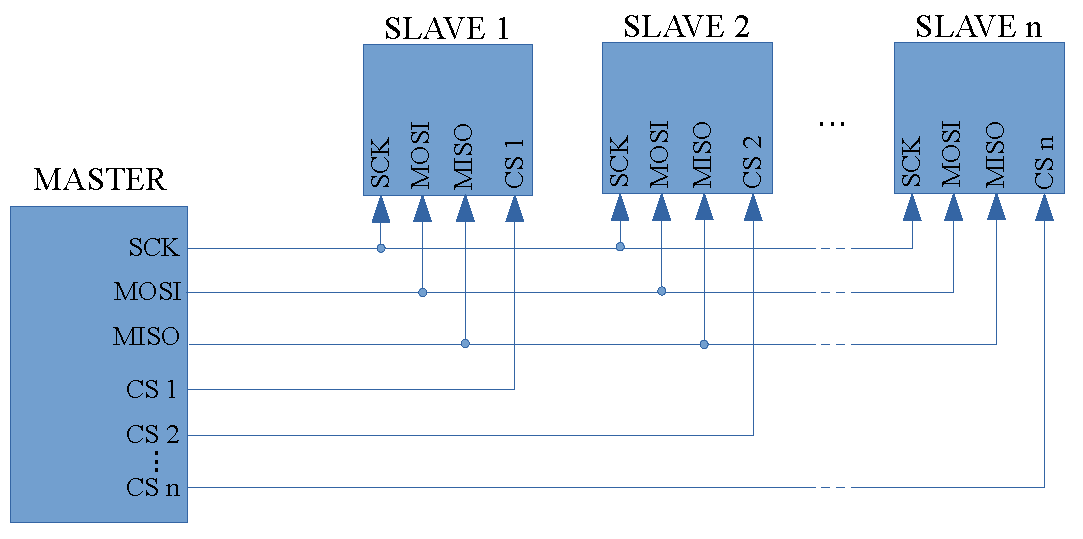
\includegraphics[width=.7\linewidth]{Assets/SPI.pdf}
	\caption{نحوه اتصال \متن‌لاتین{Slave}ها به \متن‌لاتین{Master} در حالت \متن‌لاتین{Full Duplex} }
	\label{fig:SPIWiring}
\end{figure}

سیگنال کلاک همواره توسط \متن‌لاتین{Master} تولید و به ازای هر سیگنکال کلاک یک بیت داده منتقل می‌شود. ازاین‌رو ارسال داده از \متن‌لاتین{Slave} به \متن‌لاتین{Master} به‌طور تصادفی و در هرلحظه ممکن نیست و تنها \متن‌لاتین{Slave} می‌تواند در لحظاتی که \متن‌لاتین{Master} درخواست می‌کند و سیگنال کلاک را تولید می‌کند داده را برروی خط \متن‌لاتین{MISO} ارسال کند. البته به دلیل وجود خطوط مجزای ارسال و دریافت داده، ارسال و دریافت همزمان داده نیز ممکن است. همچنین در این پروتکل دستگاه‌های \متن‌لاتین{Slave} به‌تنهایی نمی‌توانند با یکدیگر ارتباط برقرار کنند.

به جهت ارسال داده، \متن‌لاتین{Master} از طریق قراردادن خط \متن‌لاتین{SS} (یا \متن‌لاتین{CS}) در حالت \متن‌لاتین{low} انتخاب می‌کند که با کدام \متن‌لاتین{Slave} می‌خواهد ارتباط برقرار کند. وضعیت خط را تا پایان فرآیند ارسال و دریافت داده در همین حالت (\متن‌لاتین{low}) نگهمیدارد. در همین حال سیگنال کلاک را روی خط \متن‌لاتین{SCLK} متناسب با طول داده ارسالی قرار می‌دهد (ماکسیموم فرکانس کلاک بستگی به ماکسیموم مقدار قابل‌شناسایی توسط \متن‌لاتین{Slave} دارد) و داده ارسالی را نیز متناسب با کلاک روی خط \متن‌لاتین{MOSI} قرار می‌دهد (قرار دادن داده روی لبه بالارونده یا پایین‌رونده و همچنین ارسال از بیت \متن‌لاتین{MSB} یا \متن‌لاتین{LSB} بستگی به \متن‌لاتین{Slave} دارد)؛ اگر قرار باشد \متن‌لاتین{Slave} دیتایی در پاسخ به دیتای دریافتی ارسال کند (این امر باید از قبل مشخص باشد چراکه همان‌طور که گفته شد مسئول تولید کلاک فقط \متن‌لاتین{Master} است) باید \متن‌لاتین{Master} کلاک‌‌هایی متناسب با دیتای مورد انتظار برای دریافت را روی خط \متن‌لاتین{SCLK} تولید کند و دیتای مربوطه را از روی خط \متن‌لاتین{MISO} بخواند.

\قسمت{پروتکل \متن‌لاتین{I\بالانویس‌متنی{2}C}}

پروتکل \متن‌لاتین{I\بالانویس‌متنی{2}C} رابط سریالی سنکرون دو سیم است که علاوه بر پشتیبانی از چندین \متن‌لاتین{Slave} قابلیت پشتیبانی از چند \متن‌لاتین{Master} را نیز دارا می‌باشد (البته \متن‌لاتین{Master}ها قادر به برقراری ارتباط با یکدیگر نیستند و از خطوط بأس به‌طور همزمان نمی‌توانند استفاده کنند). در این پروتکل برای ارتباط از تنها دو خط سیگنال کلاک (\متن‌لاتین{SCL}\پانویس{Serial Clock Line}) و سیگنال دیتا (\متن‌لاتین{SDA}\پانویس{Serial Data Line}) استفاده می‌شود. نحوه اتصال دستگاه‌ها در این پروتکل در شکل \رجوع{fig:I2CWiring} آمده است.

\begin{figure}[!h]
	\centering
	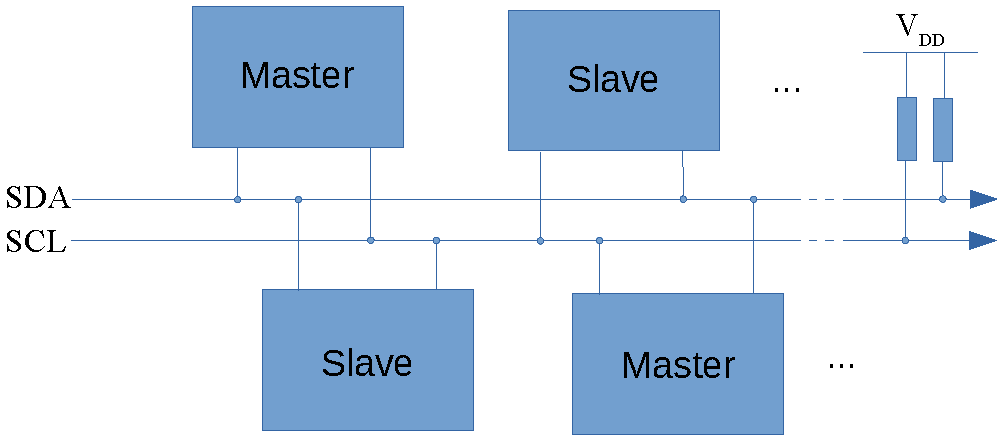
\includegraphics[width=.7\linewidth]{Assets/I2C.pdf}
	\caption{نحوه اتصال در پروتکل \متن‌لاتین{{I\بالانویس‌متنی{2}C}}}
	\label{fig:I2CWiring}
\end{figure}

در این پروتکل نیز همانند پروتکل \متن‌لاتین{SPI} سیگنال کلاک توسط \متن‌لاتین{Master} کنترل می‌شود. اعلام شروع ارسال داده با بالا نگهداشتن خط \متن‌لاتین{SCL} و پایین کشیدن خط \متن‌لاتین{SDA} انجام می‌شود. اگر دو \متن‌لاتین{Master} به‌طور همزمان قصد تبادل داده با \متن‌لاتین{Slave}ها را داشته باشند هرکدام که زودتر \متن‌لاتین{SDA} را پایین بکشید اجازه استفاده از خط را دارد و \متن‌لاتین{Master} دیگر باید تا پایان تبادلات \متن‌لاتین{Master} اول صبر کند.

برای انتقال داده پس از اعلام شروع ارسال توسط \متن‌لاتین{Master}، 7 بیت آدرس \متن‌لاتین{Slave} که قرار است با آن ارتباط برقرار شود ارسال می‌شود و پس‌ازآن یک بیت \متن‌لاتین{read/write} ارسال می‌شود تا \متن‌لاتین{Slave} از قصد \متن‌لاتین{Master} برای خواندن (سطح منطقی 1) یا نوشتن (سطح منطقی 0) مطلع شود (امکان ارتباط با \متن‌لاتین{Slave} با آدرس‌های 10 بیتی نیز وجود دارد که نحوه ارسال آن کمی متفاوت است ولی فرآیندهای دیگر در دریافت و ارسال داده‌ها یکسان است). در تمام طول ارسال و دریافت داده سیگنال کلاک نیز به‌طور منظم روی خط \متن‌لاتین{SCL} تولید می‌شود. بعد از ارسال آدرس توسط \متن‌لاتین{Master}، \متن‌لاتین{Slave}ها آدرس ارسالی را با آدرس خود مقایسه کرده و درصورتی‌که با آن مطابقت داشت بیت تصدیق (\متن‌لاتین{ACK}) را با پایین کشیدن \متن‌لاتین{SDA} تا قبل از کلاک نهم ارسال می‌کنند. اگر بیت تصدیق در این زمان ارسال نشود و \متن‌لاتین{SDA} در سطح \متن‌لاتین{high} بماند ارسال داده متوقف می‌شود چراکه عدم دریافت بیت تصدیق نشان‌دهنده عدم وجود \متن‌لاتین{Slave} موردنظر روی خط و یا عدم توانایی \متن‌لاتین{Slave} در رمزگشایی داده ارسالی است. 

پس از ارسال آدرس و دریافت تصدیق از سمت \متن‌لاتین{Slave} با توجه به بیت \متن‌لاتین{read/write} ارسالی، داده توسط \متن‌لاتین{Slave} (درحالت خواندن) و یا \متن‌لاتین{Master} (در حالت نوشتن) روی خط \متن‌لاتین{SDA} قرار داده می‌شود. بعد از ارسال هر 8 بیت داده نیز لازم است بیت تصدیق دریافت داده‌ها (\متن‌لاتین{ACK}) از طرف دریافت‌کننده داده‌ها ارسال شود. بعد از ارسال یا دریافت تمام داده‌ها باید وضعیت توقف اعلام شود تا دیگر \متن‌لاتین{Master}ها بتوانند پس‌ازآن از خط استفاده کنند. اعلام وضعیت توقف با یک تغییر وضعیت \متن‌لاتین{SDA} از سطح منطقی 0 به 1 و پس‌ازآن یک تغییر وضعیت از سطح منطقی 0 به 1  روی خط \متن‌لاتین{SCL} انجام می‌شود.

\قسمت{پروتکل USB}\label{sec:usb}

پروتکل \متن‌لاتین{USB} یک پروتکل ارتباطی سریال آسنکرون\پانویس{Asynchronous} (ناهمزمان) دو سیم است که ارتباطی بین چندین دستگاه جانبی یا \متن‌لاتین{Device} و دستگاه اصلی یا \متن‌لاتین{Host} را فراهم می‌کند. \متن‌لاتین{USB} توسط یک گروه متشکل از شرکت‌های فعال در زمینه رایانه و الکترونیک ایجاد شد که هدف ساخت پروتکل سریال همه‌منظوره برای اتصال لوازم جانبی به رایانه را داشتند. به دلیل همه‌منظوره بودن \متن‌لاتین{USB} استفاده از این پروتکل دارای جزئیات بسیار زیادی است و برخلاف دو پروتکل قبلی راه‌اندازی این پروتکل ممکن است زمان‌بر باشد. در این پروژه از این پروتکل برای ارتباط دستگاه سمت ایستگاه با رایانه و همچنین تأمین تغذیه آن استفاده می‌شود. نحوه اتصال دستگاه‌ها به \متن‌لاتین{Host} در شکل \رجوع{fig:USBConnection} آمده است.

\begin{figure}[!h]
	\centering
	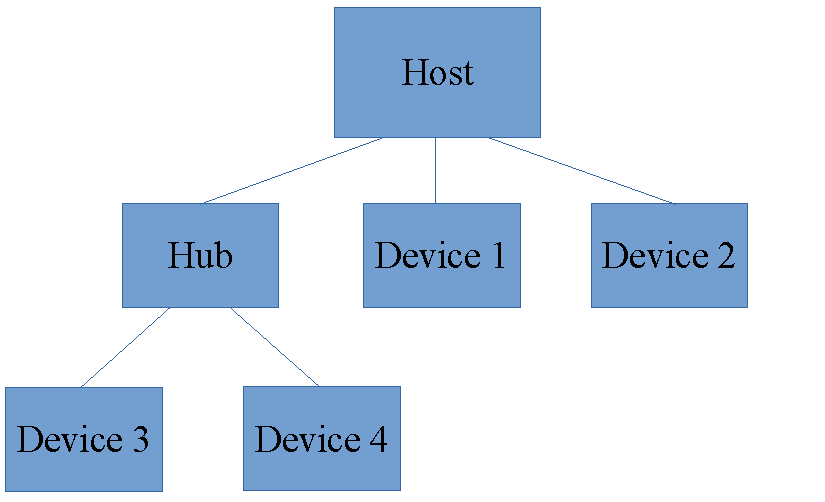
\includegraphics[width=.7\linewidth]{Assets/USB.pdf}
	\caption{نحوه اتصال دستگاه‌های جانبی به دستگاه اصلی در پروتکل \متن‌لاتین{USB}}
	\label{fig:USBConnection}
\end{figure}

به‌طورکلی برای ارتباط دستگاه‌های جانبی با دستگاه اصلی، دستگاه جانبی نیازمند دارا بودن \متن‌لاتین{Device Class} مشخص و شناخته‌شده برای دستگاه اصلی است. پیاده‌سازی دیوایس کلاس‌های اختصاصی به خاطر پیچیدگی‌هایی که این پروتکل دارد امری بسیار زمان‌بر خواهد بود به همین دلیل معمولاً استفاده از دیوایس کلاس‌های آماده (و لایبرری‌های متناطر با آن) برای ساخت دستگاه‌های جدید مناسب‌ترین روش ممکن است (این کار همچنین امر دریافت گواهی‌های سخت‌افزاری و نرم‌افزاری \متن‌لاتین{USB} را نیز تسهیل می‌کند).

در این پروتکل 4 نوع انتقال داده وجود دارد. انتقال \متن‌لاتین{Control} که تنطیمات و مشخصات دستگاه و دستورات را منتقل می‌کند. انتقال \متن‌لاتین{Isochronous} که برای انتقال داده‌هایی که زمان‌بندی در آنها اهمیت دارد نظیر صدای میکروفون و تصویر وب‌کم مورداستفاده قرار می‌گیرد. انتقال \متن‌لاتین{Bulk} که برای ارسال داده‌های حجیم‌تر به‌صورت یکجا مورداستفاده قرار می‌گیرد مانند انتقال تصویر برای پرینت و یا اسکن و یا انتقال داده‌های ذخیره‌شده روی یک فلش مموری. انتقال \متن‌لاتین{Interrupt} که داده‌هایی با حجم بسیارکم و اهمیت زیاد را جابجا می‌کند که معمولاً توسط موس، کیبرد و جواستیک (\متن‌لاتین{Joystick}) و عموماً در کلاس \متن‌لاتین{HID}\پانویس{Human interface device} مورداستفاده قرار می‌گیرد.

در این پروتکل لازم است دستگاه اصلی از تمامی جزئیات کارکرد و مشخصات دستگاه جانبی مطلع شود. مشخصات کلی دستگاه مثل ورژن \متن‌لاتین{USB} مورداستفاده، شناسه ونام سازنده، شناسه ونام دستگاه و مشخصات کلاس دستگاه در بخشی با عنوان \متن‌لاتین{Device Descriptor} با فرمتی خاص و مشخص به اطلاع رایانه می‌رسد. بخش دیگری با عنوان \متن‌لاتین{Configuration Descriptors} بیان‌کننده نحوه تغذیه و ماکسیموم توان موردنیاز دستگاه متصل به \متن‌لاتین{USB} است. بخش \متن‌لاتین{Interface Descriptors} نیز بیان‌کننده ویژگی‌های کلاس دستگاه است و شامل چندین \متن‌لاتین{Endpoint Descriptors} می‌شود که برای انجام آن ویژگی‌ها موردنیاز هستند. برای هر \متن‌لاتین{Endpoint} در سمت دستگاه جانبی ازنظر سخت‌افزاری معمولاً یک رجیستر یا مموری تعریف می‌شود که دیتا با توجه به مشخصات هر \متن‌لاتین{Endpoint} از آن خوانده می‌شود یا در آن نوشته می‌شود هر \متن‌لاتین{Endpoint} فقط مسئول یکی از اعمال خوانده شدن یا نوشته شدن است و برای هر دو عمل خواندن و نوشتن به دو \متن‌لاتین{Endpoint} نیاز است. ماکسیموم می‌توان 16 \متن‌لاتین{Endpoint} تعریف کرد، \متن‌لاتین{Endpoint} صفر رزرو و برای مشخصات کنترلی استفاده می‌شود دیگر \متن‌لاتین{Endpoint}‌ها را می‌توان با مشخات موردنیاز تعریف کرد. 

به‌طور مثال در این پروژه از کلاس \متن‌لاتین{CDC}\پانویس{Communications Device Class} استفاده‌شده است (که در کارت‌های شبکه و مودم‌ها نیز مورداستفاده قرارمی‌گیرد). برای تبادل داده با رایانه در این کلاس از ارسال نوع \متن‌لاتین{Bulk} استفاده می‌شود. پس اینترفیسی از نوع \متن‌لاتین{CDC} باید یک \متن‌لاتین{Endpoint} با دیتاتایپ \متن‌لاتین{Bulk} به‌عنوان ورودی و یک \متن‌لاتین{Endpoint} دیگر با دیتاتایپ \متن‌لاتین{Bulk} به‌عنوان خروجی داشته باشد. آدرس \متن‌لاتین{Endpoint} ورودی \متن‌لاتین{0x01} و \متن‌لاتین{Endpoint} خروجی \متن‌لاتین{0x81} تنظیم‌شده‌اند. همچنین چون قصد استفاده از \متن‌لاتین{USB} در حالت \متن‌لاتین{Full Speed} راداریم ماکسیموم سایز بسته ارسالی نیز 64 بایت تنظیم شده است. 